%%% Preamble
\documentclass[11pt]{article}

\usepackage[paper=A4,pagesize]{typearea}
\usepackage[utf8]{inputenc}
\usepackage[T1]{fontenc}
\usepackage[a4paper,pdftex]{geometry}	% Use A4 paper margins
\usepackage[french]{babel}
\usepackage{xcolor} % Required for specifying custom colors
\usepackage{fix-cm} % Allows increasing the font size of specific fonts beyond LaTeX default specifications
\usepackage{hyperref}
\usepackage{todonotes}
\usepackage{wrapfig}
\usepackage{pdfpages}
\usepackage{afterpage}
\usepackage{csvsimple}
\usepackage{float}
\restylefloat{table,figure}

%%  ========   IMPORTANT ========
%% Indiquer ici les parties que vous voulez compilez

%%% Begin document
\begin{document}
\includepdf[pages={1}]{title.pdf}

\listoftodos[Modifications du rapport]
\newpage

\tableofcontents

\listoffigures

\listoftables

\newpage

\section{Introduction}

\todo{Introduction ici}

\section{Grammaire du langage lutin}

\todo{Texte pour introduire la grammaire}

\begin{table}[h]
	\centering
	\begin{tabular}{|c|l c l|}
		\hline
		Numéro & \multicolumn{3}{c|}{Règle} \\
		\hline
		1 & P & $\rightarrow$ & D I \\
		2 & D & $\rightarrow$ & D D’ \\
		3 & D & $\rightarrow$ & $\epsilon$ \\
		4 & D’ & $\rightarrow$ & var V ; \\
		5 & D’ & $\rightarrow$ & const C ; \\
		6 & V & $\rightarrow$ & V , id \\
		7 & V & $\rightarrow$ & id \\
		8 & C & $\rightarrow$ & C , id = val \\
		9 & C & $\rightarrow$ & id = val \\
		10 & I & $\rightarrow$ & I I’ \\
		11 & I & $\rightarrow$ & I’ \\
		12 & I’ & $\rightarrow$ & lire id ; \\
		13 & I’ & $\rightarrow$ & ecrire E ; \\
		14 & I’ & $\rightarrow$ & id := E ; \\
		15 & E & $\rightarrow$ & E + E \\
		16 & E & $\rightarrow$ & E * E \\
		17 & E & $\rightarrow$ & E - E \\
		18 & E & $\rightarrow$ & E / E \\
		19 & E & $\rightarrow$ & ( E ) \\
		20 & E & $\rightarrow$ & id \\
		21 & E & $\rightarrow$ & val \\
		\hline
	\end{tabular}
	\caption{Grammaire du langage lutin}
\end{table}

\section{Automate LR}

\todo{Scan du diagramme de l'automate LR ici}

\section{Table des transitions LR}

\todo{Table des transitions ici}

%% Section : Structures de données
\afterpage{
	\clearpage
	\KOMAoptions{paper=A3,pagesize,paper=landscape,DIV=20}
	\recalctypearea
	\section{Structures de données}

	\todo{Texte pour décrire le diagramme}	
	
	\begin{figure}[h]
		\centering
		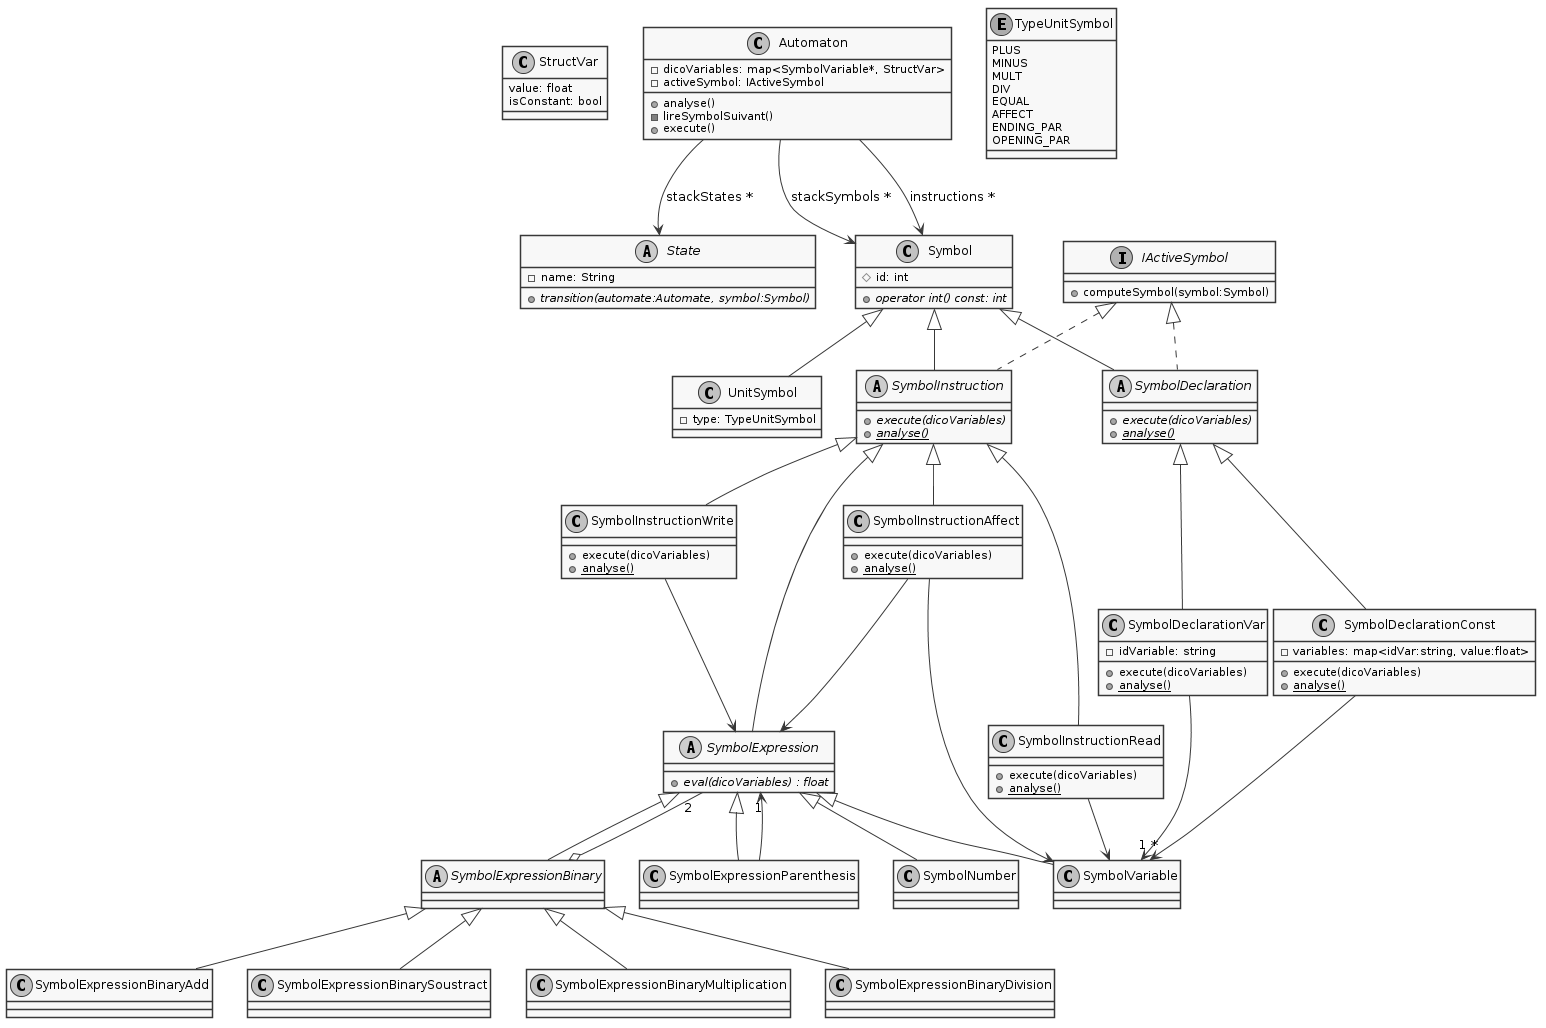
\includegraphics[width=1.0\textwidth,keepaspectratio]{../diagrams/class/lutin-compiler-class-diagram-uml.png}
		\caption{Diagramme de classe des structures de données}
	\end{figure}

	\clearpage
	\KOMAoptions{paper=A4,pagesize}
	\recalctypearea
}

%%% End document
\end{document}
